% relay on Codex whitepaper: one page. Build: see README.md in this folder.
\documentclass[9pt,a4paper]{extarticle}
\usepackage[a4paper,top=8mm,bottom=7mm,left=14mm,right=14mm]{geometry}
\usepackage[T1]{fontenc}
\usepackage[sc]{mathpazo}
\usepackage[scaled=0.9]{helvet}
\usepackage{amsmath,amssymb}
\usepackage{microtype}
\usepackage{graphicx}
\usepackage{multicol}
\usepackage{xcolor}
\usepackage{enumitem}
\usepackage[hidelinks]{hyperref}
\usepackage{titlesec}

\definecolor{ink}{HTML}{0B0B0B}
\definecolor{ink2}{HTML}{52514E}
\definecolor{accent}{HTML}{2A78D6}
\color{ink}
\hypersetup{pdftitle={Relay on Codex: running coding-agent plans across ChatGPT usage windows},pdfauthor={cube-digital}}

\setlength{\columnsep}{6mm}
\setlength{\parindent}{0pt}
\setlength{\parskip}{1.6pt}
\linespread{1.0}
\titleformat{\section}{\sffamily\bfseries\fontsize{9.2}{11}\selectfont}{\color{accent}\thesection}{0.5em}{}
\titlespacing*{\section}{0pt}{3.5pt}{1pt}
\setlist{nosep,leftmargin=1.05em,labelsep=0.45em}
\newcommand{\para}[1]{\textsf{\textbf{#1}}\enspace}
\pagestyle{empty}

\begin{document}

{\sffamily\bfseries\fontsize{15.5}{18}\selectfont Relay on Codex: running coding-agent plans across ChatGPT usage windows\par}
\vspace{2pt}
{\sffamily\small\color{ink2} cube-digital \enspace·\enspace relay codex-math v0.2 \enspace·\enspace October 2026 \enspace·\enspace Codex CLI 0.163.0, read with REA 6.7.0 and measured on a live account \enspace·\enspace \href{https://github.com/cube-digital/relay}{github.com/cube-digital/relay}\par}
\vspace{3pt}

{\small Relay turns a written plan into parallel work for the cheapest model that can do each task and keeps the plan running across usage windows. This page is the Codex counterpart of the relay whitepaper: what the Codex harness meters and exposes (recovered from the binary, checked on a live Business account), what that changes in relay's mechanism, the model behind the Codex forecast, and what the first measurements say. Facts and evidence: \textsf{codex-math/config/codex-harness.json}, \textsf{codex-math/evidence/}; model code: \textsf{codex-math/lib/}.\par}

\vspace{2pt}
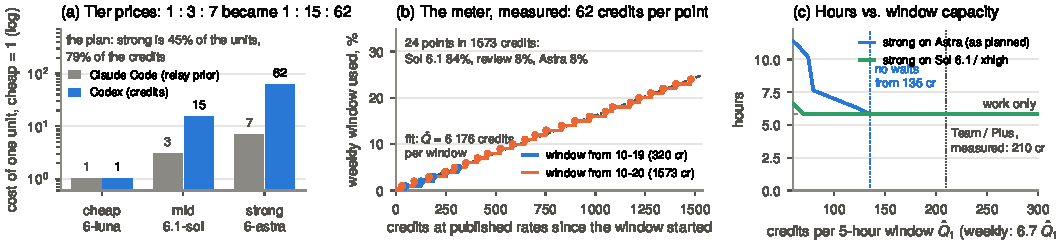
\includegraphics[width=\textwidth]{figure.pdf}
{\footnotesize\color{ink2} \textbf{Figure 1.} (a)~The relay whitepaper's 30-task plan (7 lanes, 3 waves, 108.4 units, 4.7 expected fix rounds) on Codex: credits per unit by tier, Luna\,:\,Sol~6.1\,:\,Astra $=1:15:62$ at the measured token mix and meter weights, where relay's Claude prior was $1:3:7$; the plan's strong tasks are 45\% of its units and 79\% of its 131 credits. (b)~The meter, measured: a Business account's weekly window against the credits its threads spent at the published rates, two windows, 29 integer steps, $\hat Q=6\,176$ credits per window, i.e.\ 62 credits per point. (c)~Hours for the plan against the 5-hour capacity $\hat Q_1$: at the measured Team capacity of 210 credits it runs its 5\,h\,51\,min with no pause (none above 135 credits); with the strong tier on Sol~6.1/xhigh it costs 66 credits. Computed by \textsf{data.mjs} with the model code.\par}

\begin{multicols}{2}
\fontsize{8.0}{9.45}\selectfont

\section{What the harness meters}
Read from \textsf{@openai/codex} 0.163.0 with REA: process captures of the binary (help, \textsf{exec -{}-json}, the TUI, the app-server over stdio), its protocol schema and model catalog, the strings of its \textsf{.rodata}, two defaults decompiled from its code; then checked on a live Business account (\textsf{self\_serve\_business\_prolite}): 114 rollouts mined, nine priced runs, a spawn-limit run. The credit rates are OpenAI's published ones.
\begin{itemize}
\item \para{Windows are plan-shaped, not fixed.} A reading is a \textsf{RateLimitSnapshot}: \textsf{primary} and \textsf{secondary} windows with \textsf{usedPercent}, \textsf{resetsAt} and \textsf{windowDurationMins}, plus \textsf{planType}, \textsf{credits} and a per-pool view keyed by \textsf{limit\_id}. Team meters a 5-hour and a weekly window; Pro and the Business plan measured here only the weekly one. \textsf{usedPercent} is an integer; an unused window's \textsf{resetsAt} slides with the clock until the first metered use, and a mid-window reset shows as a changed \textsf{resetsAt}. Readings come from \textsf{account/rateLimits/read} (and \textsf{/updated}) on the app-server and from the \textsf{token\_count} event in each rollout file; API-key sessions get none.
\item \para{Credits are the unit, with weights.} Published rates per million tokens, input\,/\,cached\,/\,output: Luna 2.5\,/\,0.25\,/\,12.5, Sol~6.1 50\,/\,2.5\,/\,250, Astra 250\,/\,25\,/\,1250; Fast meters $2.5\times$ the included usage ($2\times$ purchased credits) for a 1.5--2$\times$ speedup; Ultrafast $8\times$. The weekly window moved linearly in these credits (Fig.~1b, residual 0.6 points) with one correction: Astra work counts about half its published rate (0.43--0.57, five steps). The backend's per-thread estimate (\textsf{account/usage/read \{threadId\}}) is \textsf{null} on this plan, so the published rates are the only per-thread price.
\item \para{Tokens are attributable.} Every subagent is its own thread: \textsf{state\_5.sqlite} holds its model, effort and token total, \textsf{thread\_spawn\_edges} its parent; \textsf{exec -{}-json} ends with \textsf{turn.completed.usage}. Real sessions are 97\% cached input by tokens. The usable context is 95\% of the window (258\,400 tokens; Sol~6.1 got a 500\,k window from the remote catalog on 14~October); auto-compaction triggers at 90\% of the window (244\,800, decompiled); tool output is cut at 10\,000 tokens; compaction is hookable (\textsf{PreCompact}, \textsf{PostCompact}).
\item \para{Levers relay did not have.} Spawns take \textsf{model}, effort and speed; \textsf{[agents]} sets the subagent defaults and \textsf{max\_concurrent\_threads\_per\_session} the children (default 3: the compiled limit is 4 threads with the root, and the 4th spawn fails with \emph{agent thread limit reached}); a \textsf{PreToolUse} hook can rewrite a \textsf{spawn\_agent} call through \textsf{updatedInput} (the Codex form of relay's mod); reset credits restore every window at once; a thread \emph{goal} with a token budget keeps an idle thread going until \textsf{budget\_limited} or \textsf{usage\_limited} (relay's marathon, built in).
\end{itemize}

\section{What changes in the mechanism}
Tiers keep their roles, but the ladder is $1:15:62$, so the cheap tier is nearly free: Luna costs $1/15$ of Sol per unit, still $1/5$ at three times the turns; Astra is spent only where the plan says strong. Lanes run at most three abreast unless \textsf{[agents]} raises the limit. Budget gates degrade in price order: speed to standard, effort to medium, then strong to mid; the architect is exempt at tight; a weekly window is gated by the weekly lines wherever the account reports it. A reset credit is spent when the next pause exceeds an hour. The ledger stamp carries the account's windows and the credits spent: \textsf{[primary 23.4\% resets 16:30 · secondary 41\% · credits 12.5]}.

\section{The model}
\para{Units.} As in relay, task $t$ weighs $w_t=T(\text{tier}_t)R(\text{risk}_t)$ with $T=(1,3,7)$, $R=(0.8,1,1.4)$, read now as relative token volume. On tier $\tau$ a unit processes $\nu_\tau$ tokens (prior 70\,k) in the measured shares $\alpha=(0.03,0.965,0.005)$ of uncached input, cached input and output; with the model's rates $p_\tau$, its meter weight $\omega_\tau$ (Astra 0.5, else 1), the speed multiplier $s_\tau$ and the effort multiplier $e_\tau$ on output, a unit costs
\[
c_\tau=\omega_\tau s_\tau\,\nu_\tau\,(\alpha_{\mathrm{in}}p^{\mathrm{in}}_\tau+\alpha_{\mathrm{c}}p^{\mathrm{c}}_\tau+\alpha_{\mathrm{out}}e_\tau p^{\mathrm{out}}_\tau)/10^6
\]
credits: 0.027, 0.41 and 1.65 at the priors, which is what nine scratch runs of 1--3 units measured (0.018--0.026, 0.30--0.49, 0.74). Lane $l$ costs $C_l=\sum_{t\in l}w_t c_{\tau(t)}$.

\para{Fix rounds.} Unchanged: lane $l$ needs a fix round with probability $p_l\in\{0.2,0.5,0.8\}$ re-working $\kappa=0.35$ of it, so $\tilde C_l=C_l(1+\kappa p_l)$, $\mathrm{E}[C]=\sum_l\tilde C_l=131$ and $\mathrm{Var}[C]=\kappa^2\sum_l C_l^2p_l(1-p_l)$, $\mathrm{SD}=8.4$; the exact distribution over the $2^7$ outcomes agrees.

\para{Windows.} Window $j$ holds $Q_j$ credits, so the plan uses $U_j=\mathrm{E}[C]/Q_j$ of it: 62\% of a Team 5-hour window ($Q_1=210$), 9\% of its week ($Q_2=1\,400$), 2\% of a Business week ($Q=6\,176$). The walk runs a wave while every window is below its stop line ($85\%$ primary, $95\%$ secondary), spends credits and time linearly, pauses at a line until that window resets, rolls windows over on schedule, and spends a reset credit instead of a long pause when one is available. Wave time is $m\,M_k$ with $M_k$ the makespan of the lanes' expected units on three slots; Fast divides a lane's minutes by its speedup and multiplies its credits by 2.5, which prices the trade per wave (wave 1 saves 32\,min for 10 credits, wave 2 saves 93\,min for 102).

\para{Calibration} has two layers that never share a parameter. Capacity: between two readings with no reset, the credits spent and the points the window moved give $\hat Q_j=100\sum\Delta C/\sum\Delta u_j$, a ratio estimator over all such intervals, independent of the plan; readings of concurrent threads are pooled on the account's credit timeline against each window's high-water mark, which made Fig.~1b from a machine's rollouts before relay ran at all. Price per unit: every lane thread's credits are known, so $\hat c_\tau=\sum C/\sum w$ over the threads on tier $\tau$, at one model, effort and speed; with only wave totals, non-negative least squares of $\Delta C_k$ on the units per tier. Time: $\hat m=\sum\Delta t_k/\sum M_k$ as before. Each estimate replaces its prior from the first sample.

\section{What is not claimed}
\begin{itemize}
\item Measured once, on one machine: $\hat Q$ for the Business week (29 steps, two windows, days within 10\%), Team's 5-hour and weekly windows (two windows each: 212/277 and 1\,300/1\,640 credits; usage on other devices is invisible to a rollout and biases $\hat Q$ low), Pro's week (four steps, 12\,600--18\,100); Plus is assumed equal to Team. $\nu_\tau$, $e_\tau$, $T$, $R$, $p_l$ and $\kappa$ are still priors: the scratch runs were too small to show effort in the output, and a relay unit has not been timed on Codex.
\item The meter weights are relative to Sol~6.1 and fitted where the account ran other models; Luna's is unmeasurable there (5 credits) and left at 1. Rates and catalog change without a binary change (Sol~6.1's window did); a mid-thread model, effort or speed change re-reads the context at the uncached rate.
\item Lanes are independent and front-load usage less than real runs do; the walk ignores spend controls and pools other than the primary \textsf{limit\_id}. Savings are not measured yet: next, ten calibrated waves, then an A/B of the same plans on Codex plain and with relay.
\end{itemize}

{\scriptsize\color{ink2}
Evidence: \textsf{codex-math/evidence/} (REA captures, schemas, catalog, SQLite DDL, \textsf{.rodata} strings; \textsf{live/}; \textsf{decompile/}; \textsf{RESULTS.md}); docs cited in \textsf{codex-harness.json}. Rebuild: \textsf{docs/whitepaper/README.md}.\par}

\end{multicols}
\end{document}
